% ============================================
% Second column, Techniques and samples
% ============================================

\separatorcolumn

\begin{column}{\colwidth}

    \begin{alertblock}{Measuring strain in three dimensions}

        Bragg Coherent Diffraction Imaging relies on:

        \begin{itemize}
            \setlength\itemsep{1em}
            \item Highly coherent synchrotron sources.
            \item Samples below coherent volume: \qty{\approx 1}{\um^3}.
            % \item The beam must be very intense and focused since the samples are very small.
            % \item High setup stability, possibility to go probe high angles, in many different directions.
            \item Highly faceted samples.
        \end{itemize}

        \begin{figure}
            \includegraphics[width=0.45\textwidth]{/IntroductionMIT/BraggLaw.png}
            \includegraphics[width=0.45\textwidth]{/IntroductionMIT/StrainedCrystal.png}
        \end{figure}

        \centering
        Access to \textbf{full displacement field} \textrightarrow Defect identification!

    \end{alertblock}

    \begin{block}{Sample preparation}

        \begin{columns}[T]
            \begin{column}{0.6\colwidth}
                \begin{figure}
                    \centering
                    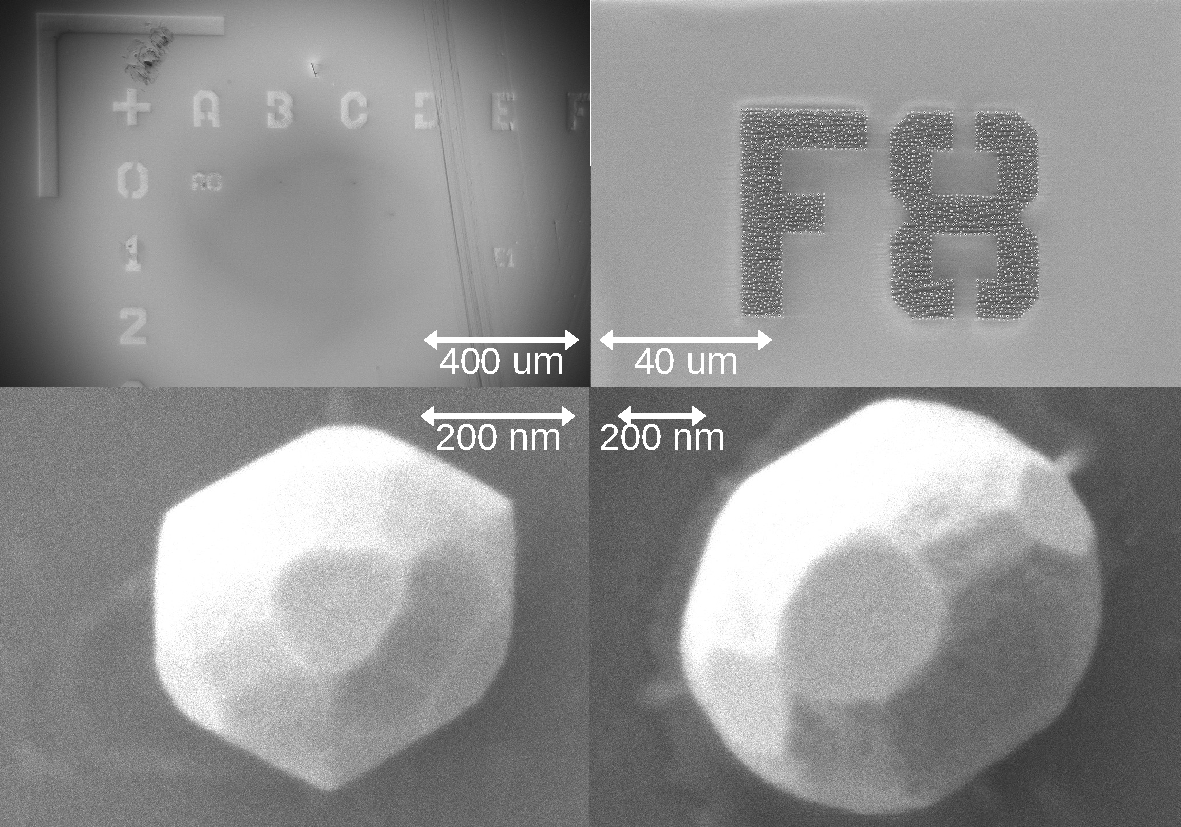
\includegraphics[width=0.575\colwidth]{MITSamples/Char/SEM/SEM_Poster.pdf}
                    \caption{EBL pattern and Ni particles imaged by scanning electron microscopy.}
                    \label{fig:EBLPattern}
                \end{figure}
            \end{column}

            \begin{column}{0.4\colwidth}
                \begin{enumerate}
                    \item Pattern drawn by electron beam lithography (EBL).
                    \item Crystallization by annealing in forming atmosphere.
                    \item SEM imaging and EBSD crystal orientation determination.
                \end{enumerate}

            \end{column}

        \end{columns}

    \end{block}

    \begin{block}{Sample characterisation}

        \heading{The interface plays a crucial role in the supported crystals shape, orientation, and strain field.}

        \begin{table}[htb]
            \centering
            \resizebox{\textwidth}{!}{%
                \begin{tabular}{@{}lllllll@{}}
                \toprule
                Substrate  & \ce{Nb}:\ce{SrTiO3}(001) & \ce{SiO2}(001)(1 ML)& \ce{SiO2}(001)(2 ML)& \ce{SiO2}(001)( 3ML)& \ce{SiO2}(001) & Si(001) \\
                 &  & /Si(001) & /Si(001) & /Si(001) &  & \\
                \midrule
                $W_{\text{sep}}$ (\unit{\J/\meter^2})  & 0.19 & 0.61 & 0.70 & 1.60 & 2.16 & 3.16 \\
                 $\gamma_{int}$ (\unit{\J/\meter^2})  & 2.76 & -- & -- & -- & 2.92 & 0.97 \\
                 \bottomrule
                \end{tabular}%
            }
            \caption{Work of separation $W_{\text{sep}}$ and interfacial energies ($\gamma_{int}$) for Ni(111) on different substrates.}
            \label{tab:wos_gamma_table}
        \end{table}

        \begin{figure}
            \centering
            \includegraphics[width=\colwidth]{MITSamples/Char/TEM/TEM_DFT.pdf}
            \caption{a) Cross-sectional TEM image of a Ni particle on \ce{SiO2} / \ce{Si}(001) substrate.
            b) Zoom on interphase boundary with c) EDS measurement and d) Interface schematic. e) DFT cell used for interface calculations in Tab. \ref{tab:wos_gamma_table}.}
        \end{figure}

        \begin{figure}
            \centering
            \includegraphics[width=\colwidth]{MITSamples/Char/SXRD/InPlaneMaps.pdf}
            \caption{
            In-plane reciprocal space maps of Ni dewetted on \ce{SiO2} covered [001] oriented \ce{Si} (left), and [001] oriented \ce{Nb}:\ce{SrTiO3} (right).
            }
        \end{figure}

    \end{block}

    \begin{block}{\textit{In situ} corrosion cell}
        \begin{figure}
            \centering
            \includegraphics[width=0.9\colwidth]{/ElectrochemicalCell/Fig_ABCD.pdf}
            \caption{Electrochemical cell design, compatible with three electrode setup, liquid flow, and four different synchrotron beamlines.}
        \end{figure}
    \end{block}

\end{column}
